\section{Inhalt}

% REPLACE FILES IN THIS DIRECTORY WITH YOUR OWN CONTENT

\subsection{Akronyme}

Das ist ein \gls{acr}.
Diese kann man in dem \gls{glossary} finden.

\subsection{Abbildungen}

In \autoref{fig:exampleImage} wird ein Beispielbild gezeigt.

\begin{figure}[h]
    \centering
    \includegraphics[width=0.8\textwidth]{test.jpg}
    \caption[Beispielbild]{Beispielbild von \citeauthor{exampleImage} aus \autocite{exampleImage}.}
    \label{fig:exampleImage}
\end{figure}

In \autoref{fig:exampleFigure} wird eine Beispielgraph dargestellt.

\begin{figure}[h]
    \centering
    \begin{subfigure}{0.45\textwidth}
        \begin{tikzpicture}
            \begin{axis}[width=1.0\textwidth]
            \addplot[color=red]{exp(x)};
            \end{axis}
        \end{tikzpicture}
        \caption{Expontentialfunktion in 2D}
        \label{fig:2d-exp}
    \end{subfigure}
    \begin{subfigure}{0.45\textwidth}
        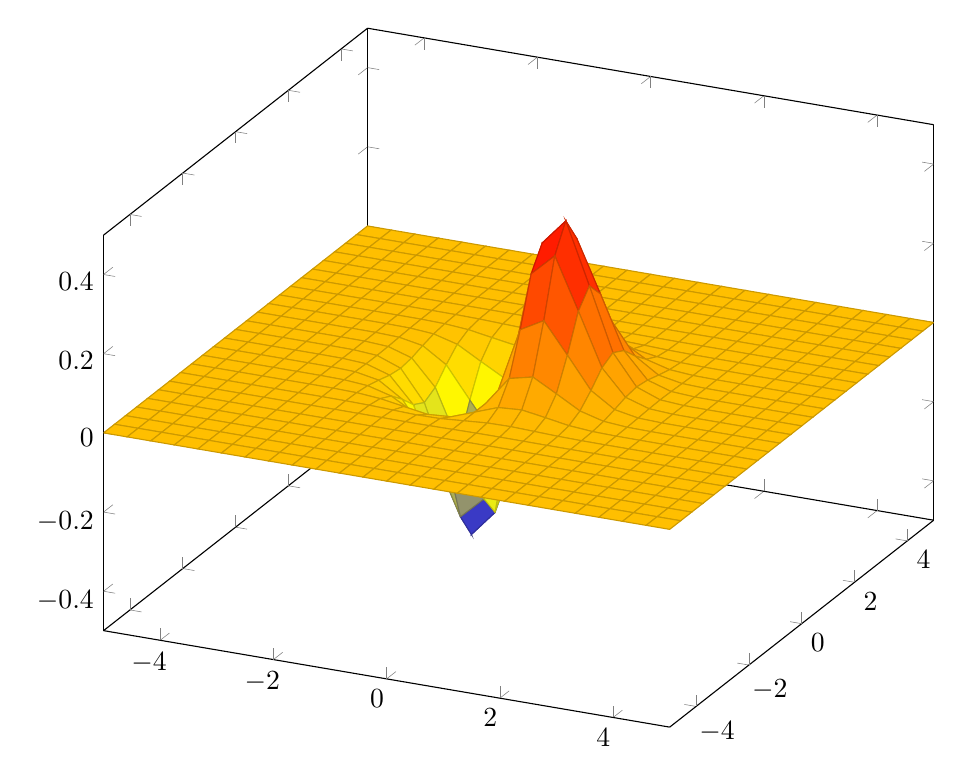
\begin{tikzpicture}
            \begin{axis}[width=1.0\textwidth]
                \addplot3[surf]{exp(-x^2-y^2)*x};
            \end{axis}
        \end{tikzpicture}
        \caption{Expontentialfunktion in 3D}
        \label{fig:3d-exp}
    \end{subfigure}
    \caption[Beispielgraph]{Beispielgraph in \textsc{pfgplots}.}
    \label{fig:exampleFigure}
\end{figure}

\subsection{Tabelle}

Es folgt nun eine Tabelle in \autoref{tab:exampleTable}.

\begin{table}[h]
    \centering
    \begin{tabular}{|l|l|}
        \hline
        \textbf
        Land & Hauptstadt
        \normalfont \\
        \hline
        \hline
        Deutschland & Berlin\\
        \hline
        Simbabwe & Harare\\
        \hline
        Grönland & Nuuk\\
        \hline
    \end{tabular}
    \caption{Beispieltabelle}
    \label{tab:exampleTable}
\end{table}

\subsection{Tikz}

In \autoref{fig:tikz} wird eine CircuitTi\textit{k}Z Zeichnung dargestellt.

\begin{figure}[h]
    \centering

    \begin{circuitikz}[]
    \draw (0,0) to[short, o-] (2,0) to[R,l_=$R_1$] (2,-2) to[short,*-o] (3,-2);
    \draw (2,-2) to[R,l_=$R_2$, -*] (2,-4);
    \draw (0,-4) to[short, o-o] (3,-4);
    \draw (0,0) to[open, l=$U_{\text{in}}$] (0,-4);
    \draw (3,-2) to[open, l=$U_{\text{out}}$] (3,-4);
    \end{circuitikz}

    \caption{Beispielschaltung}
    \label{fig:tikz}
\end{figure}

\subsection{Mathe}

Die Riemannsche Zeta-Funktion ist in \autoref{eq:exampleEquation} aufgeführt.

\begin{equation}
\begin{gathered}
\zeta(s) = \sum_{n=1}^{\infty} \frac{1}{n^s} = \frac{1}{1^s} + \frac{1}{2^s} + \frac{1}{3^s} + \ldots \\[2ex]
\text{für } \Re(s) > 1 \text{ und dessen analytischer Kontinuation}
\end{gathered}
\label{eq:exampleEquation}
\end{equation}

Eine Demonstration des modifizierten Wurzel Symbols ist in \autoref{eq:sqrt} gezeigt.

\begin{equation}
    c = \sqrt{a^{2} + b^{2}}
    \label{eq:sqrt}
\end{equation}

\subsection{Quellcode}

In \autoref{code:exampleCode} ist Quellcode gezeigt.
In \autoref{code:latex} wird Quellcode aus einer Datei angezeigt.

\begin{lstlisting}[
    language=C,
    caption={Ein einfacher C code}, language=C++, label=code:exampleCode, float=h
]
#include <stdlib.h>
#include <stdio.h>

int main(void)  {
    printf("Hello World!\n");
    return EXIT_SUCCESS;
}
\end{lstlisting}

\lstinputlisting[
    linerange={127-134},
    firstnumber=127,
    caption={\texttt{./content.tex} Beispiel zum Einbetten von Quellcode aus einer Datei},
    language=TeX,
    label=code:latex,
    float=h
]{./text/content.tex} %path is relative to main document.tex

\subsection{Timing Diagramm}

In \autoref{fig:timingFig} ist ein Timing Diagramm abgebildet.

\begin{figure}[h]
    \begin{center}
    \begin{tikztimingtable}[%
        timing/dslope=0.2,
        timing/.style={x=1.6ex,y=2ex},
        x=1ex,
        timing/rowdist=4ex,
        timing/c/rising arrows,
        timing/name/.style={font=\sffamily\scriptsize},
    ]
    % Draw tikztimingtable signals
    \busref{CS} & HHL;16{L};LHH\\
    \busref{SCK} & UULL;16{C};UU\\
    \busref{SO} & UUU;2D{D7};2D{D6};2D{D5};2D{D4};2D{D3};2D{D2};2D{D1};2D{D0};UUU\\
    % Add verticals bars to background
    \extracode
    \begin{pgfonlayer}{background}
        \begin{scope}[semitransparent ,semithick]
            \vertlines[darkgray,dotted]{0,3.2 ,...,36.0}%
        \end{scope}
    \end{pgfonlayer}
    \end{tikztimingtable}
    \end{center}
    \caption{Zeitablauf einer Datenübertragung}
    \label{fig:timingFig}
\end{figure}

\subsection{Text}
Der folgende Text ist ein Auszug aus \textit{Wikipedia} zu der Demonstration der Leichtigkeit der Lesbarkeit des Satzes.

Der Fauststoff, genannt auch Faust-Sage, die Geschichte des Doktor Johann Faust und seines Pakts mit Mephistopheles, gehört zu den am weitesten verbreiteten Stoffen in der europäischen Literatur seit dem 16. Jahrhundert. Das lückenhafte Wissen über den historischen Johann Georg Faust\footnote{wohl etwa 1480-1541} und sein spektakuläres Ende begünstigten Legendenbildungen und ließ Schriftstellern, die sich mit seinem Leben befassten, einigen Spielraum. Eigenschaften des Fauststoffs, die in den unterschiedlichsten Versionen wiederkehren, sind Fausts Erkenntnis- oder Machtstreben, sein Teufelspakt und seine erotischen Ambitionen.

Während sich in der Populärkultur ältere Vorstellungen von Faust als Narr und Scharlatan hielten, geschah seit dem 18. Jahrhundert eine literarische Aufwertung des Fauststoffs. Der menschliche Zwiespalt zwischen der Kraft des Glaubens und der Sicherheit wissenschaftlicher Erkenntnis wurde zu einem Hauptthema. Faust ist der über seine Grenzen hinaus strebende Mensch und befindet sich im Konflikt zwischen egozentrischer Selbstverwirklichung und sozialer Anerkennung in einer stets noch religiös geprägten Welt.
Es folgt nun ein Lorem Ipsum.

\lipsum[1]

\subsubsection{Thema}
\lipsum[2-4]
\subsubsection{Thema}
\lipsum[5-7]

